\graphicspath{{chapters/09/images/}}
\chapter{Vascularization}

\section{Angiogenesis and pore size}
Angiogenesis is the bottleneck of tissue engineering.
In order to regenerate functional tissues, stimulation, control or inhibition of angiogenesis are critical.
The porosity of the scaffold is fundamental for promoting vascularization.
A broad distribution of pore sizes and pore shapes ranging from very small to very large can be required.

	\subsection{A case regarding pore size}
	In fig \ref{fig:pores} is described the design of a very simple porous scaffold.
	This scaffold has been built combining polymers with spheres: holes filled with water and then emptied.
	The ratio between spheres and solution has to be tuned carefully.
	Black holes in the image are interconnections.
	Another technique to build such a scaffold is salt leaching, where we first add crystals to polymeric solution and then salt is removed.
	The regular shape is kept fixed thanks to crystal dimensions.
	In the case of spherical pores, the interconnection depends on the number of spheres per volume.
	Size and interconnection can be modulated by selecting the concentration.

	\begin{figure}[h]
		\centering
		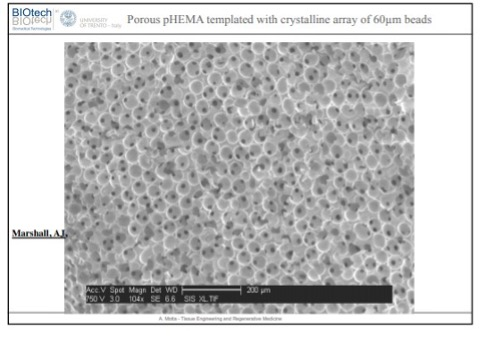
\includegraphics[width=0.5\textwidth]{pores}
		\caption{\label{fig:pores}}
	\end{figure}

	The black dots representing interconnections have a dimension of $5$ micron.
	By playing with the scaffold, different families of pores can be obtained.
	In the case of smaller pores more capillaries are obtained.
	The ideal range for the black dots is between 40 and 50 microns.
	The highest vascular density was observed in the case of smaller porosity, between 0 and 100 micrometers.
	Very large porosity leads to the formation of a layer of endothelial cell with no 3D tube required for vascularization.

\section{Scaffold vascularization strategies}
Different strategies can be employed to vascularize a scaffold.

	\subsection{Growth factor delivery}
	The delivery of single or multiple angiogenic GF to stimulate loading molecules can be performed by mixing with the polymer allowing for a fast release.
	To slow the release they can be included in a drug releasing system like polymeric nanoparticles.
	In this way the release of the factors will be tied with the degradation time of those nanoparticles.
	This factors can also be linked to the molecules to the polymeric chain.
	This strategies can be combined to allow for a sequential release of different factors.

	\subsection{Cell transplantation}
	In cell transplantation cells and extracellular matrix are grown outside the body and then implanted to promote vascularization.

	\subsection{Scaffold pre-vascularization}
	Robust tubes in the scaffold are produced in order to anastomize with osteoblasts.
	Factors to attract already existing vascular tubes to the scaffold can be used.

	\subsection{Decellularized  scaffold}
	A human derived, decellularized myocardium not populated by endothelial cells is used to promote vascularization.
	The main difficulty in this strategy is to guarantee a very low amount of DNA.
	There is a need to check that no debris is left after decellularization to avoid thrombogenesis through forced migration to reform endothelium.

	\subsection{Angiogenic biomaterial}
	An angiogenic biomaterial is the best option if possible.
	The biomaterial is designed such that it is able to induce vascularization per se.
	These are called “precision biomaterials”, as they are designed to have a specific function.
	They can be nature derived biomaterial like proteins derived from silk that have intrinsic angiogenic potential or synthetic functionalized biomaterials.

	\subsection{Microfabrication methods}
	Microfabrication methods are a top-down approach: they built the vessels and around them the tissue.
	Decellulariziation can be skipped by directly inserting endothelial cells.

\section{Angiogenic potential evaluations}
In vitro procedures should be carefully designed, to obtain useful considerations on the scaffold.
Consider figure \ref{fig:coculture}: mononuclear cells are seeded inside the hydrogel upon isolation of two main endothelial progenitor cells populations from peripheral blood.
Cells were seeded and checked after 4 and 10 days.
In the case of IKVAV modified culture there is more signals.
This means there are more cells, more clusters and more layers due to migration.
The aim was to design a precision material to be used in brain, laminin derived to mimic the brain ECM.
The strategy consisted of isolation of peptides involved in differentiation and linking them to polymeric chain.
During angiogenesis tubes are expected to form, but this didn't happened, because the in vitro model was too far from physiology: the cell are not in a monolayer.
Changing the model cells were able to drive tube formation.

\begin{figure}[h]
	\centering
	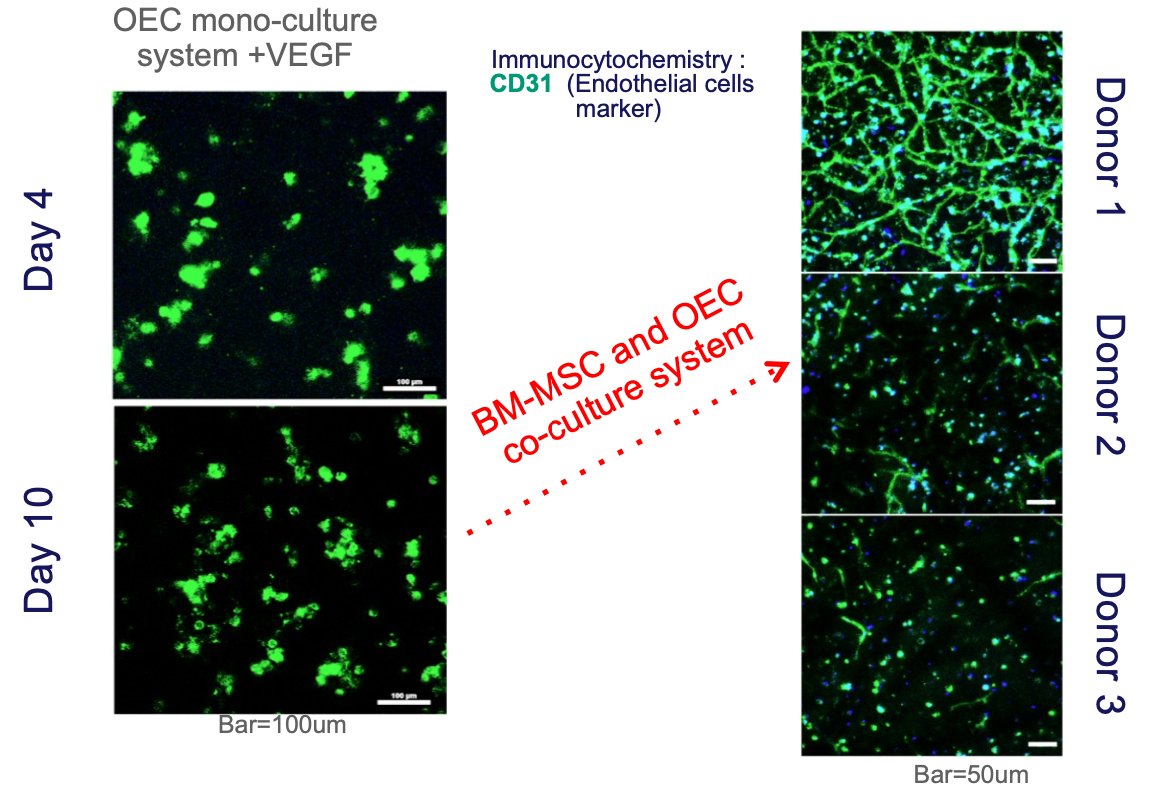
\includegraphics[width=0.5\textwidth]{coculture}
	\caption{\label{fig:coculture}}
\end{figure}

	\subsection{Stem cells}
	In studies concerning donor-derived stem cells at least $5$ replicates need to be used.
	The personalized solution in order to avoid variability is needed to achieve the best result.

	\subsection{Bone scaffold}
	Considering bone, the presence of two families of cells leads to the best results: osteoblast work will lead to an increase endothelial cells formation.
	This is because osteoblast cells know how much and when to release factors.
	Osteoblasts also produce a collagenic template used by endothelial cells to form tubes.
	When we take into account the scaffold, the direct interaction with both osteoblast and endothelial cells using for example fibroin micronets.
	The endothelial cells become tubes creating a collagenic network.

\section{Vascularization strategies}
To achieve better blood vessels architecture is important.
Endothelial cells must be fed with some molecules to amplify the angiogenesis process.
Porous matrices can be loaded with growth factor and functionalized to recruit blood vessels from surrounding tissues.
They should be able to penetrate and form interconnected tissue.
The main vascularization strategies are:

\begin{multicols}{2}
	\begin{itemize}
		\item Angiogenesis: ingrowth of vascular sprouts from the host microvasculature into implanted tissue construct, which finally form a new microvascular network.
		\item Inosculation: a pre-created vessels in vitro is generated within a tissue construct prior to implantation.
			Then a connection with host vessels and already included vessels happens.
			Usually animal cells are used in order to distinguish which vessels are new and which are implanted through staining.
			Sometimes scaffold tubes are not able to anastomize and die, the aim is to preserve the mixture and anastomize.
	\end{itemize}
\end{multicols}

\begin{figure}[h]
\centering
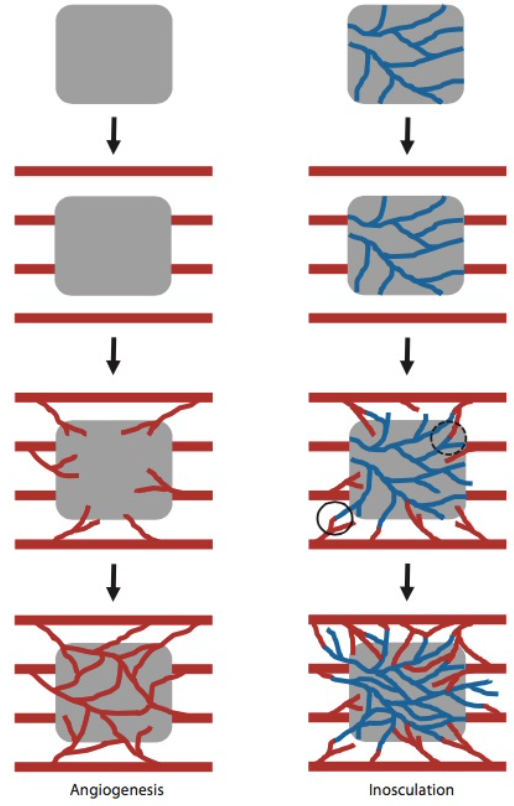
\includegraphics[width=0.3\textwidth]{vasc}
\caption{\label{fig:vasc}}
\end{figure}

	\subsection{Immune response and vascularization}
	Inflammation induces angiogenesis.
	After the recruitment of macrophages and the formation of granulation tissue this must be vascolarized.
	In the case of a high porosity structure a fine granulation tissue is found, with the presence of angiogenic factors and new vessels.
	After $2$ week the inflammatory response ha decreased.
	In the case of a less porous scaffold there is no vascularization and a thick layer of fibrotic tissue.

	\subsection{Effect of silk fibroin on vascularization}
	So, to promote vascularization the polymer should form a sponge, like:

	\begin{multicols}{2}
		\begin{itemize}
			\item PDLLA: blood vessels are just around after $3$ weeks.
			\item PDLLAA and silk fibers: there is a very nice capillary branch formation into the scaffold after $3$ weeks.
		\end{itemize}
	\end{multicols}

	After 6 weeks silk seems to be intrinsically angiogenic.
	The best scaffold will always be the one with the quickest angiogenesis.

	\begin{figure}[h]
		\centering
		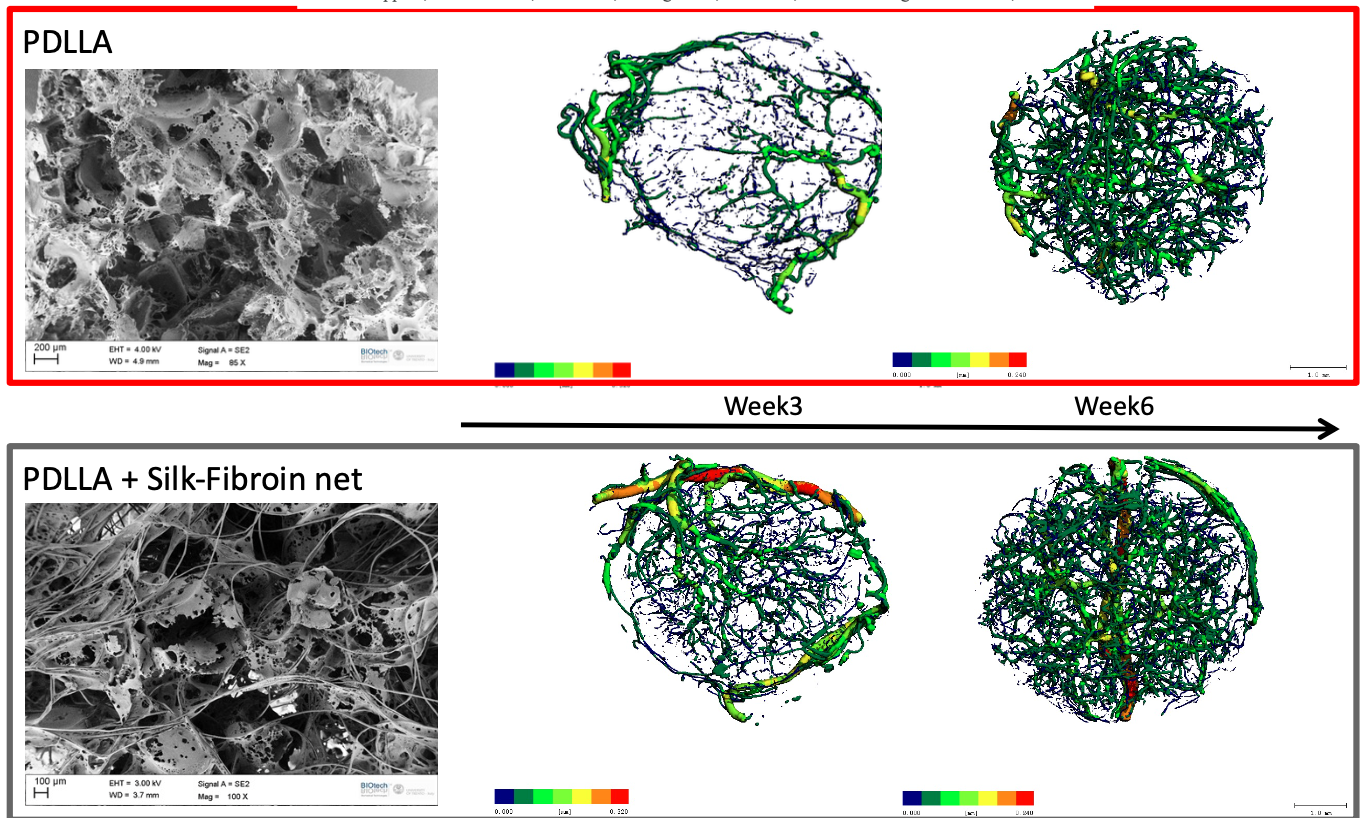
\includegraphics[width=0.5\textwidth]{pdlla}
		\caption{\label{fig:pdlla}}
	\end{figure}


	\subsection{Angiogenesis driven by inflammatory cells}
	In this experiment the fibroin net was implanted with and without pre-seeding osteoblasts.
	A very nice and intense angiogenesis was observes thanks to the interaction between osteoblasts and inflammatory signal.
	Different pre-culture time show that the inflammatory response better in the case B.
	The second scaffold has a better angiogenesis.
	Because of this it can be said that the drug release system works and speeds up the angiogenesis process.

	\begin{figure}[h]
		\centering
		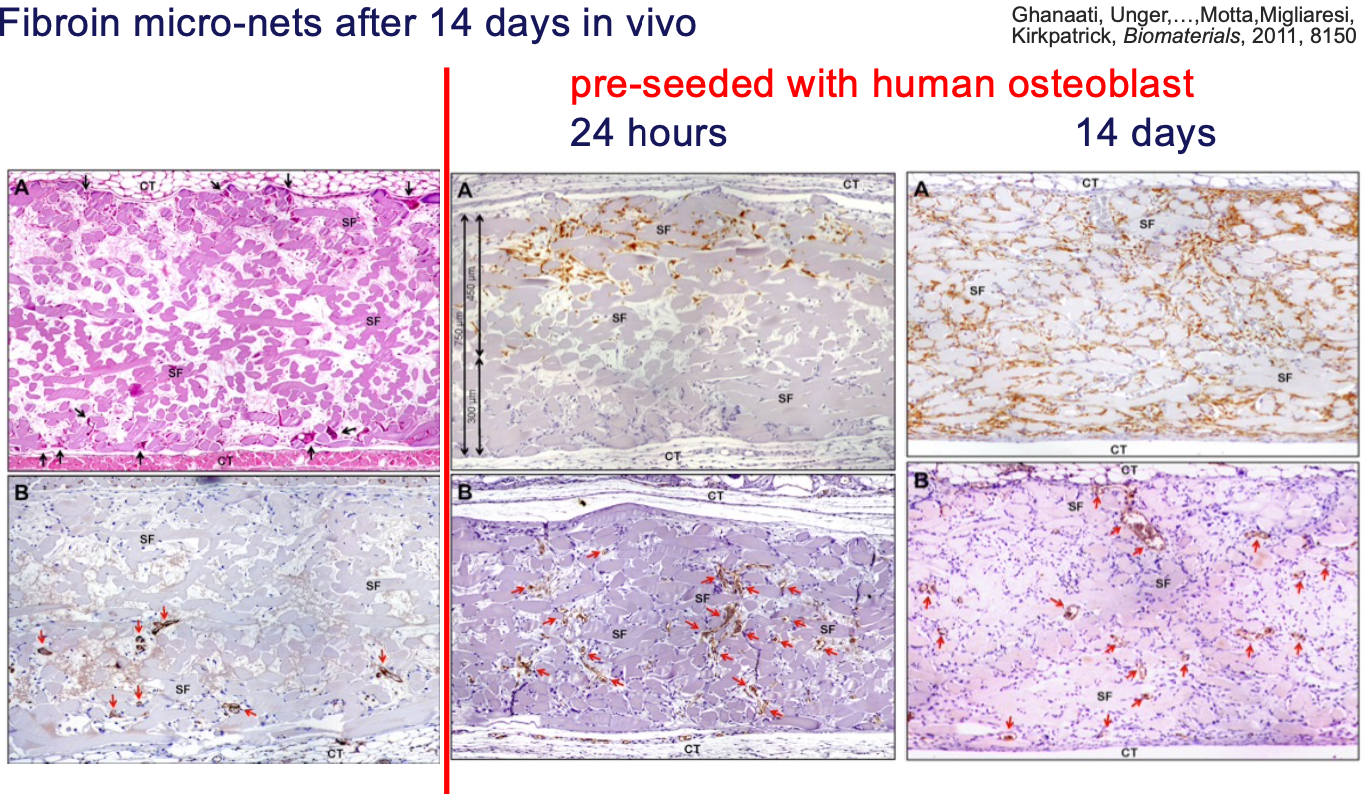
\includegraphics[width=0.5\textwidth]{fibroin}
		\caption{\label{fig:fibroin}}
	\end{figure}

\section{Induction of vascularization in TE scaffolds}
After the selection and dosage of the molecules necessary to promote angiogenesis how to release them into the system must be decided.

	\subsection{PDGF-containing microspheres}
	A dual factor delivery from degradable scaffolds for de novo blood vessels synthesis can use PDGF-containing microspheres.
	The molecules must exit from the vescicles, move in a matrix and then release in a very slow process.
	The fact that degradation does not occur prior to release and wheter microparticles are active and alive throughout the waiting needs to be assessed.

	\subsection{Cytokine delivery}
	The sequential delivery of VEGF and PDGF-BB using a controlled release polymeric device subcutaneously and in hind limb ischemia model induced a mature new vascular network with vessels having a thick coat of smoot muscle cells.
	The combination of the two gives the best and fastest angiogenesis.

	\subsection{Microparticles}
	Scaffold design by microparticle assembly.
	Microparticles preparation:

	\begin{multicols}{2}
		\begin{itemize}
			\item Formation of microparticles via single emulsion.
			\item Double emulsion with growth factors.
		\end{itemize}
	\end{multicols}

	This methods includes microspheres loaded or not with drugs.

		\subsubsection{Sintering}
		Sintering is the formation of microparticles with some porosity inside.
		Single emulsion is a method of sintering.
		The sintering process allows for a good adhesion.
		It is usually used for metallic-alloy, polymers and ceramics.
		The porosity can be controlled by mixing the solution iwth water.

		\subsubsection{Printing}
		Microparticles are printed.

	\subsection{Strategies for enhancing vascularization}

	\begin{table}[H]
		\centering
		\begin{tabular}{|c|c|c|}
			\hline
			& By host & Engineered vascular network\\
			\hline
			\multirow{2}{*}{Pros} & Easy to engineer & Immediate perfusion\\
														& High quality vessels &\\
			\hline
			\multirow{3}{*}{Cons} & Too slow & Hard to engineer\\
														& 				 & Compatibility\\
														& 				 & Needs tubes\\
			\hline
		\end{tabular}
		\caption{Pros and cons of strategies for enhancing vascularization}
	\end{table}
